\documentclass[english,14pt]{beamer}
\usetheme{EastLansing}
\usecolortheme{spruce}

\usepackage{xcolor}
\usepackage{listings}
\usepackage{courier}
\usepackage{graphicx}
\usepackage{amsmath}
\usepackage{algorithm2e}
\usepackage{multicol}
\usepackage{hyperref}
\usepackage{textcomp}

% http://mirrors.ibiblio.org/CTAN/macros/latex/contrib/datetime2/datetime2.pdf
\usepackage{babel}
\usepackage[useregional]{datetime2}

% https://tex.stackexchange.com/questions/42619/x-mark-to-match-checkmark
\usepackage{pifont}% http://ctan.org/pkg/pifont

%% https://stackoverflow.com/questions/1435837/how-to-remove-footers-of-latex-beamer-templates
%%gets rid of bottom navigation bars
%\setbeamertemplate{footline}[page number]
%
%gets rid of navigation symbols
\setbeamertemplate{navigation symbols}{}


\usefonttheme[onlymath]{serif}

\definecolor{mGreen}{rgb}{0,0.6,0}
\definecolor{mGray}{rgb}{0.5,0.5,0.5}
\definecolor{mPurple}{rgb}{0.8,0,0.82}
\definecolor{backgroundColour}{rgb}{0.95,0.95,0.92}
\definecolor{lightBlue}{rgb}{0.1, 0.1, 0.8}
\definecolor{darkGreen}{rgb}{0, 0.39, 0}

\newcommand\red[1]{{\color{red} #1}}
\newcommand\green[1]{{\color{green} #1}}
\newcommand\blue[1]{{\color{blue} #1}}
\newcommand\darkGreen[1]{{\color{darkGreen} #1}}

\newcommand{\cmark}{\ding{51}}%
\newcommand{\xmark}{\ding{55}}%

\lstdefinestyle{CStyle}{
    backgroundcolor=\color{backgroundColour},   
    commentstyle=\color{mGreen},
    keywordstyle=\color{magenta},
    numberstyle=\tiny\color{mGray},
    stringstyle=\color{mPurple},
    basicstyle=\footnotesize,
    breakatwhitespace=false,         
    breaklines=true,                 
    captionpos=b,                    
    keepspaces=true,                 
    numbers=left,                    
    numbersep=5pt,                  
    showspaces=false,                
    showstringspaces=false,
    showtabs=false,                  
    tabsize=2,
    language=Python
}

\lstdefinestyle{pseudo}{
        basicstyle=\ttfamily\footnotesize,
        keywordstyle=\color{lightBlue},
        morekeywords={BEGIN,END,IF,ELSE,ENDIF,ELSEIF,PRINT,WHILE,RETURN,ENDWHILE,DO,FOR,TO,IN,ENDFOR,BREAK,INPUT,CONDITIONS},
        morecomment=[l]{//},
        commentstyle=\color{mGreen}
}

\lstset{basicstyle=\footnotesize\ttfamily,breaklines=true}
\lstset{framextopmargin=50pt,tabsize=2}

\title{ENGG1003 - Thursday Week 8}
\subtitle{Numerical integration }%\\ \& computing integrals}
\author{Steve Weller}
\institute{University of Newcastle}
%\date{\today}
\date{29 April 2021}

% following is a bit of a hack, but forces page numbers (technically: frame numbers) to run 1,2,3,... 
% with titlepage counting as frame 1

\addtocounter{framenumber}{1}
\titlepage

\begin{document}

\begin{flushleft}
{\scriptsize Last compiled:~\DTMnow}
\vspace*{-5mm}
\end{flushleft}
\framebreak

%==============================================================

\begin{frame}[fragile]

\frametitle{Lecture overview}
\begin{enumerate}
	\item Basic ideas of numerical integration \red{\S6.1}
	\begin{itemize}
		\item engineering applications
		\item terminology \& notation
		\item additivity
	\end{itemize}
	
	\item[]
	
	\item Trapezoidal method \red{\S6.2}
	
%	\item[]
%	
%	\item Midpoint method, upper/lower and left/right Riemann sums \red{\S6.3}
	
	\item[]
	
	\item Simpson's rule
	
\end{enumerate}

\end{frame}

%==============================================================

\begin{frame}[fragile]

\frametitle{$1)$ Basic ideas of integration}

% https://en.wikipedia.org/wiki/File:Integral_as_region_under_curve.svg
\vspace*{-5mm}
\begin{figure}[ht]
	\centering
	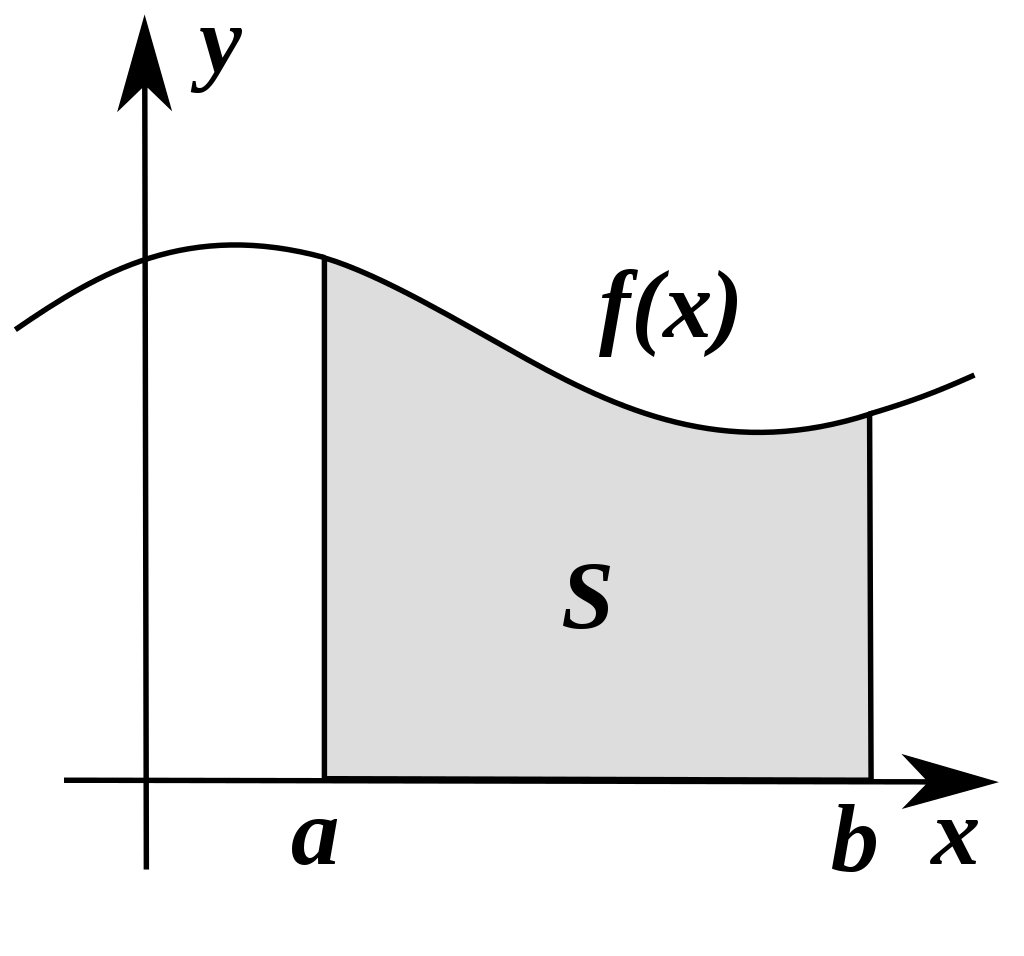
\includegraphics[width=0.35\textwidth]{figures/integralArea}
\end{figure}
\vspace*{-5mm}
\[
S = \int_a^b f(x) dx
\]
\vspace*{-5mm}
\begin{itemize}
	\item area $S$ is area under function $f(x)$ between lower limit $a$ and upper limit $b$
	\item assume $f(x) \geq 0$
	\item calculus, eg: MATH1002, MATH1110
\end{itemize}

\end{frame}

%==============================================================

\begin{frame}[fragile]

\frametitle{Engineering applications of integration}

% https://www.whitman.edu/mathematics/calculus_online/chapter09.html

\begin{itemize}
	\item 1. Area between curves
2. Distance, Velocity, Acceleration
3. Volume
4. Average value of a function
5. Work
6. Center of Mass
7. Kinetic energy; improper integrals
8. Probability
9. Arc Length
10. Surface Area
\end{itemize}

\end{frame}

%==============================================================

\begin{frame}[fragile]

\frametitle{Distance $=$ area under speed-time function}

Assume that you speed up your car from rest, on a straight road, and wonder how far you go in T seconds. The displacement is given by the integral
\[
\int_0^T v(t)dt
\]
where $v(t)$ is the velocity (speed) as a function of time

Example:
\[
v(t) = 3t^2e^{t^3}
\]

\end{frame}

%==============================================================

\begin{frame}[fragile]

\frametitle{}

\begin{figure}[ht]
	\centering
	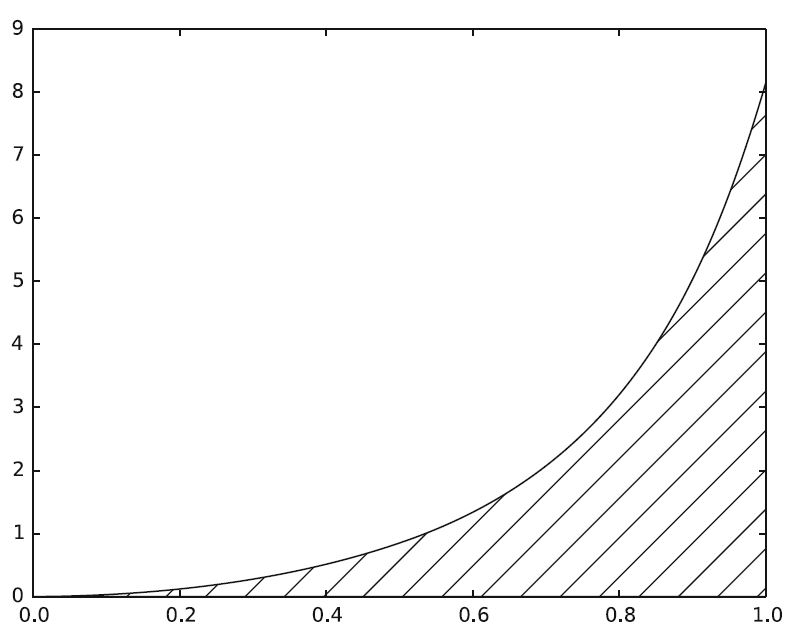
\includegraphics[width=0.5\textwidth]{figures/LLp134}
\end{figure}

distance traveled in first second is cross-hatched area:
\[
\int_0^1 v(t)dt
\]

Start at time $0$, end at time $1$ (these are the lower and upper limits)
\end{frame}

%==============================================================

\begin{frame}[fragile]

\frametitle{$2)$ Trapezoidal method}

Example:
\vspace*{-5mm}
\begin{figure}[ht]
	\centering
	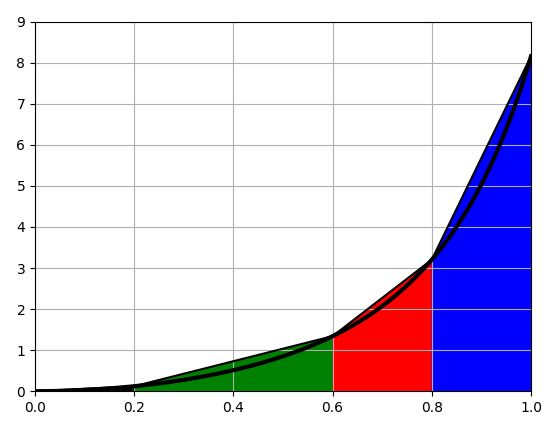
\includegraphics[width=0.5\textwidth]{figures/fourPanel}
\end{figure}
\vspace*{-3mm}
\begin{itemize}
	\item approximate area under curve by total area of four trapezoids
	\begin{itemize}
		\item black + \darkGreen{green} + \red{red} + \blue{blue}
	\end{itemize}
	\item area of each trapezoid is easy to calculate %: $\frac{a+b}{2} h$
\end{itemize}



\end{frame}

%==============================================================

\begin{frame}[fragile]

\frametitle{Area of trapezoid}

\begin{itemize}
	\item area of trapezoid $\frac{A+B}{2} h$
\end{itemize}
\vspace*{-3mm}
\begin{figure}[ht]
	\centering
	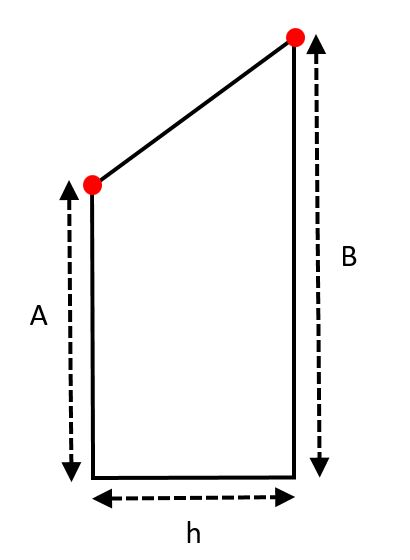
\includegraphics[width=0.4\textwidth]{figures/trapezoidArea}
\end{figure}

\end{frame}

%==============================================================

\begin{frame}[fragile]

\frametitle{}

\begin{figure}[ht]
	\centering
	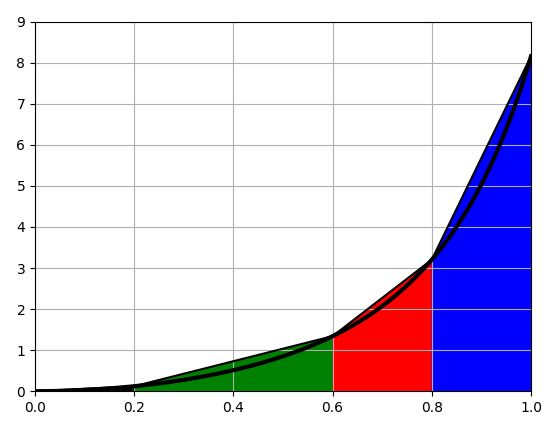
\includegraphics[width=0.5\textwidth]{figures/fourPanel}
\end{figure}
\vspace*{-5mm}
{\small
\begin{eqnarray*}
\int_0^1 v(t)dt & = & \int_0^{0.2} v(t)dt + \int_{0.2}^{0.6} v(t)dt + \int_{0.6}^{0.8} v(t)dt + \int_{0.8}^1 v(t)dt \\
\pause
&\approx & h_1 \frac{v(0) + v(0.2)}{2} + \darkGreen{h_2 \frac{v(0.2) + v(0.6)}{2}} + \\
& & +h_3 \red{\frac{v(0.6) + v(0.8)}{2}} + \blue{h_4 \frac{v(0.8) + v(1)}{2}} 
\end{eqnarray*}
}
\pause
\vspace*{-5mm}
\[
h_1 = 0.2, \quad h_2 = 0.4, \quad h_3 = 0.2, \quad h_4 = 0.2
\]

\end{frame}

%==============================================================

\begin{frame}[fragile]

\frametitle{General trapezoidal method}

\begin{itemize}
	\item want to approximate integral $\int_a^b f(x)dx$ by $n$ trapezoids \emph{of equal width}
	\begin{itemize}
		\item total of $n$ intervals: $[x_0,x_1]$, $[x_1,x_2]$, \ldots $[x_{n-1},x_n]$
	\end{itemize}
\end{itemize}

{\small
\[
\int_a^b f(x)dx = \int_{x_0}^{x_1} f(x)dx + \int_{x_1}^{x_2} f(x)dx + \cdots + \int_{x_{n-1}}^{x_n} f(x)dx
\]
\pause
\[
\approx h\frac{f(x_0)+f(x_1)}{2} + h\frac{f(x_1)+f(x_2)}{2} + \cdots + h\frac{f(x_{n-1}) + f(x_n)}{2}
\]
\pause
In compact form:
\blue{
\[
\int_a^b f(x)dx \approx h \left[ \frac{1}{2}f(x_0) + \left\{ f(x_1)+\cdots+f(x_{n-1}) \right\} + \frac{1}{2}f(x_n) \right]
\]
}}

\end{frame}

%==============================================================

\begin{frame}[fragile]

\frametitle{Python code for trapezoidal method}

\texttt{trapezoidal\_method.py}
\begin{lstlisting}[style=CStyle,basicstyle=\scriptsize]
import numpy as np

def v(t):
    return 3*t**2*np.exp(t**3)

def trapezoidal(f, a, b, n):
    h = (b-a)/n
    f_sum = 0
    for i in range(1, n, 1):
        x = a + i*h
        f_sum = f_sum + f(x)
    return h*(0.5*f(a) + f_sum + 0.5*f(b))

n = 4
trap = trapezoidal(v, 0, 1, n)
exact = np.exp(1) - 1

print('Trapezoidal, {} sub-intervals: {:.8f}'.format(n,trap))
print('Exact answer: {:.8f}'.format(exact))
\end{lstlisting}

\end{frame}

%==============================================================

\begin{frame}[fragile]

\frametitle{Trapezoidal method: simulation results}

\begin{itemize}
	\item lines 3--4: function to be integrated
	\item[]
	\item lines 6--12: function to approximate integral using $n$ trapezoids of equal width $h$
	\begin{itemize}
		\item lines 8--11: compute $f(x_1) + \cdots f(x_{n-1})$
	\end{itemize}
	\item[]
	\item line 16: exact result $\int_0^1 3t^2e^{t^3}dt = e - 1$
	\item[]
	\item live demo, try $n=4$, $n=100$ and $n=1000$ sub-intervals
\end{itemize}

\end{frame}

%%==============================================================
%
%\begin{frame}[fragile]
%
%\frametitle{$3)$ Midpoint method}
%
%\begin{itemize}
%	\item skip details, all give quite similar results to trapezoidal method, esp for narrow width panels, some details in \red{\S6.3}
%	\item[]
%	\item mention/visualise different methods:
%	\begin{itemize}
%		\item midpoint method
%		\item upper/lower Riemann sums 
%		\item left/right Riemann sums
%	\end{itemize}
%\end{itemize}
%
%\end{frame}

%==============================================================

\begin{frame}[fragile]

\frametitle{$3)$ Simpson's rule}

% https://en.wikipedia.org/wiki/Simpson%27s_rule
\begin{figure}[ht]
	\centering
	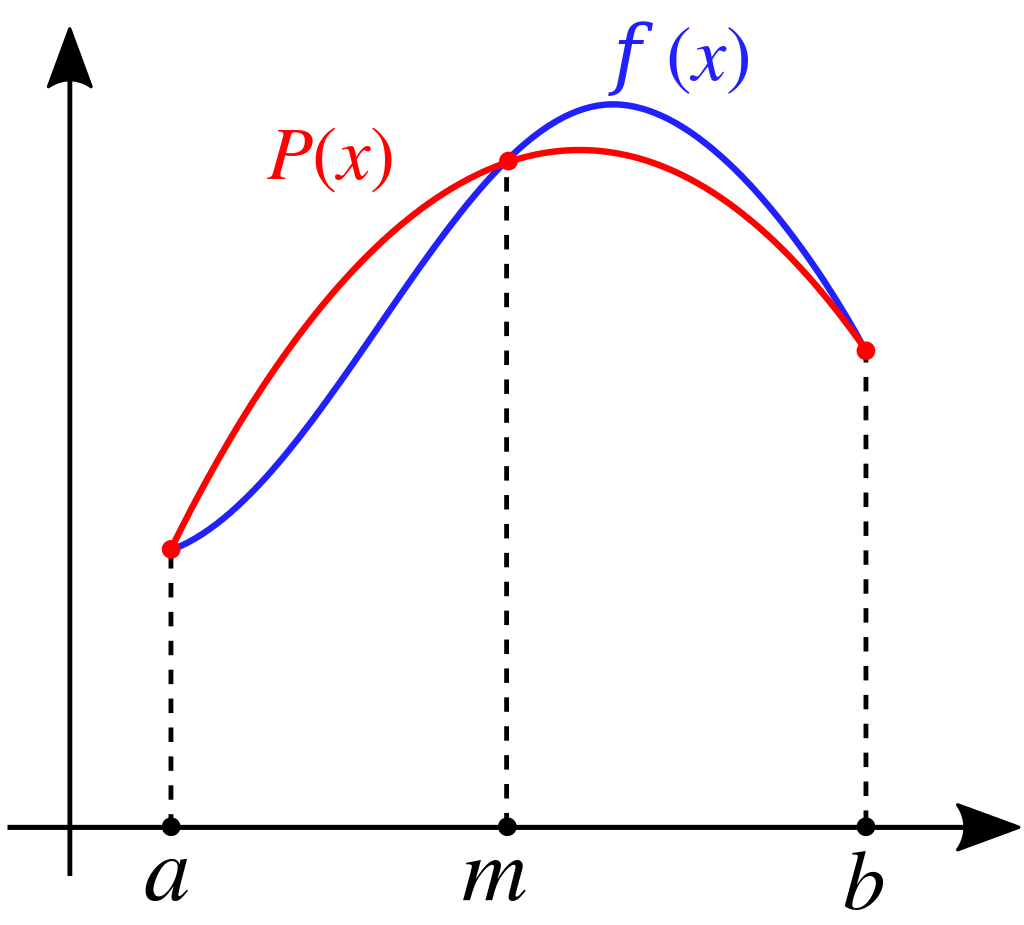
\includegraphics[width=0.4\textwidth]{figures/SimpsonsRule}
\end{figure}

\begin{itemize}
	\item approximate \blue{$f(x)$} with parabola \red{$P(x)$}
	\item parabola $P(x)$ takes same values as $f(x)$ at end-points $a$ and $b$, and midpoint $m = (a+b)/2$
\end{itemize}

\end{frame}

%==============================================================

\begin{frame}[fragile]

\frametitle{Simpson's rule}

\begin{itemize}
	\item area under parabola $P(x)$ between $a$ and $b$ is:
\[
\int_a^b P(x) dx
\]
\item[] \ldots which can be calculated \emph{exactly} for a parabola (proof omitted):

\blue{
\[
\int_a^b f(x)dx \approx \frac{b-a}{6} \left[ f(a) + 4f\left(\frac{a+b}{2}\right) + f(b)\right]
\]
}

\end{itemize}

\end{frame}

%==============================================================

\begin{frame}[fragile]

\frametitle{Applying Simpson's rule}

\begin{itemize}
\item as for trapezoidal rule, apply Simpson's rule on each sub-interval of width $h = x_i - x_{i-1} = (b-a)/n$
	\begin{itemize}
		\item total of $n$ intervals: $[x_0,x_1]$, $[x_1,x_2]$, \ldots $[x_{n-1},x_n]$
	\end{itemize}
\end{itemize}

{\small
\[
\int_a^b f(x)dx = \int_{x_0}^{x_1} f(x)dx + \int_{x_1}^{x_2} f(x)dx + \cdots + \int_{x_{n-1}}^{x_n} f(x)dx
\]
}

\end{frame}

%==============================================================

\begin{frame}[fragile]

\frametitle{Python code for Simpson's rule}
\vspace*{-2mm}
\texttt{simpsons\_rule.py}
\begin{lstlisting}[style=CStyle,basicstyle=\scriptsize]
import numpy as np

def v(t):
    return 3*t**2*np.exp(t**3)

def simpson(f, a, b, n):
    h = (b-a)/n
    x0 = a
    summ = 0
    # i-th sub-interval (i=0,1,...,n-1) is [x_i,x_{i+1}]
    for i in range(0,n,1):
        xi = x0 + i*h
        summ += (f(xi) + 4*f((xi+xi+h)/2) + f(xi+h))*h/6
    return summ

n = 4
simp = simpson(v, 0, 1, n)
exact = np.exp(1) - 1

print('Simpson, {} sub-intervals: {:.8f}'.format(n,simp))
print('Exact answer: {:.8f}'.format(exact))
\end{lstlisting}

\end{frame}

%==============================================================

\begin{frame}[fragile]

\frametitle{Simpson's rule: simulation results}

\begin{itemize}
	\item lines 3--4: function to be integrated
	\item[]
	\item lines 6--14: function to approximate integral using Simpson's rule on each of $n$ sub-intervals $[x_i,x_{i+1}], i = 0,1,2,\ldots,n-1$
	\begin{itemize}
		\item line 13: Simpson's rule with $a=x_i$ and $b=x_{i+1}$
	\end{itemize}
	\item[]
	\item live demo, try $n=4$, $n=10$ and $n=100$ sub-intervals
\end{itemize}

\end{frame}

%==============================================================

\begin{frame}[fragile]

\frametitle{Lecture summary}

\begin{enumerate}
	\item Basic ideas of integration
	
	\item[]
	
	\item Trapezoidal method \red{\S6.2}
	
%	\item[]
%	
%	\item Midpoint method \red{\S6.3}
	
	\item[]
	
	\item Simpson's rule
	
\end{enumerate}

\end{frame}

\end{document}